% =========================== ACT II: BUILD ===========================
% storyboard.md Act II. Job: AI changes what you keep -- code, and the
% documents that describe your work. Act II opens directly on Task 4, then
% gives "code -> package" real depth with a named, git-verified example,
% then closes out Task 3's proposal thread with a best-practices takeaway.
%
% Task 4 is BITS for GAPS, Dr. Kyla Jones's published paper (Computers &
% Chemical Engineering 211, 2026), converted into a public package by
% Alex after publication. Named the same way Jeff Kantor is named in the
% Prologue: real credit tied to real public authorship (first author,
% DOI'd), no invented biographical detail. The five Task 4 slides below
% are git-verified against the real `dowlinglab/bits_for_gaps` commit
% history (103 commits, all Alex, July 3 - Aug 7, 2026) and a since-
% deleted but git-recoverable `HANDOFF.md` that narrated the whole
% conversion in numbered phases (kept as sourcing evidence only -- the
% slides themselves no longer narrate by phase number, per Alex's own
% 2026-09-04 accessibility pass). emcal's own closing slide was cut the
% same day (package not complete yet, Act II needed the time back) -- see
% the comment where it used to sit, below.
\stagedivider{3}{Act II: Build}{What's worth keeping?}

% Graphical abstract cropped from the real GitHub README screenshot Alex
% captured (figures/bits_for_gaps_screenshot.png), CC BY 4.0, (c) 2026 The
% Authors -- same license terms as the README's own caption.
\begin{frame}{Task 4 --- convert code from a published paper into a package}
  \ndlogonote{\scriptsize\href{https://github.com/dowlinglab/bits_for_gaps}{\texttt{github.com/dowlinglab/bits\_for\_gaps}}}
  \vfill
  \begin{center}
    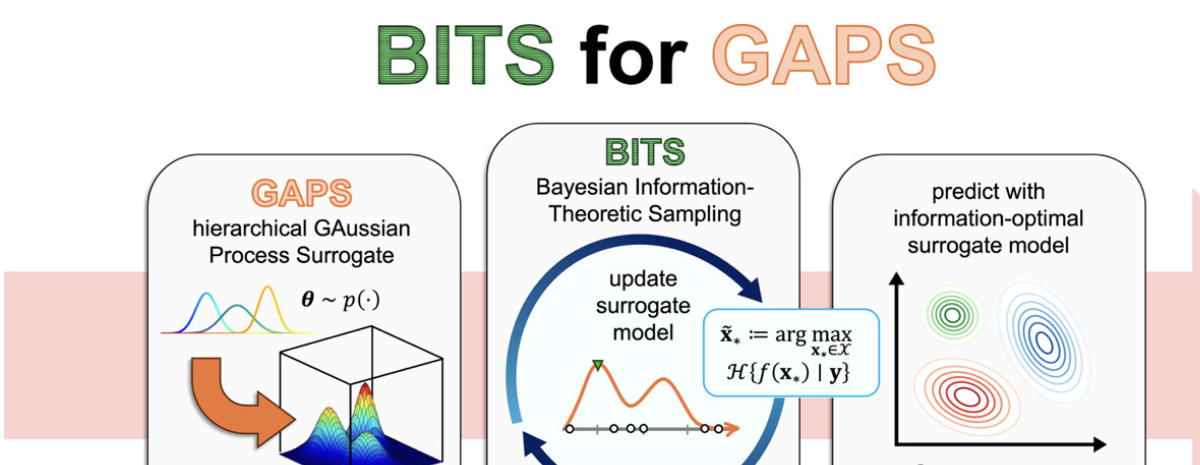
\includegraphics[width=0.56\textwidth]{figures/bits_for_gaps_graphical_abstract}\\[0.15em]
    {\scriptsize K.~D.~Jones and A.~W.~Dowling, \textit{Computers \& Chemical Engineering} \textbf{211} (2026) 109650}
  \end{center}
  \vspace{0.35em}
  \begin{center}
    \slidepoint{After Kyla defended her thesis, I turned her well-organized private codebase into a \textbf{public, pip-installable package} using Claude Code!}
  \end{center}
  \vspace{1.8cm plus 1fill}
\end{frame}

% The recipe list is reconstructed from the public dowlinglab/bits_for_gaps
% commit history and its since-deleted REFACTOR_PLAN.md (git-recoverable).
% REFACTOR_PLAN.md originally numbered ten phases, 0-9, with Phase 9 =
% Publish. After Phase 8 (docs) finished, a planning commit (4f74d46,
% 2026-07-04) split the old "Phase 9 = Publish" into a new Phase 9 (full
% stochastic reproduction) and pushed Publish to Phase 10; from there, four
% more phases were proposed live, one at a time, each only after the
% previous one had already merged: 9b (a real bug, found the same day
% Phase 9 finished), 9c, 9d, 9e -- Publish (Phase 10) didn't actually
% happen until a month after 9e merged. Thirteen labeled phases executed
% against ten planned; the four improvised ones (9b-9e) are the
% brace-highlighted items below. Same recipe, written out in prose, in
% scientific_computing_workflow.md \S2-4.
\begin{frame}{Task 4 --- the recipe, final paper code $\to$ generalized, published package}
  \ndlogonote{\scriptsize\href{https://github.com/dowlinglab/claude-for-researchers/blob/main/resources/practices/scientific_computing_workflow.md}{\texttt{resources/practices/scientific\_computing\_workflow.md}}\\[0.3em]\href{https://bits-for-gaps.readthedocs.io}{\texttt{bits-for-gaps.readthedocs.io}}}
  \vspace{-0.9cm}
  \begin{center}
  \begin{enumerate} \normalsize \setlength\itemsep{0.28em}
    \item Extract the paper's code into an installable package, not just scripts
    \item Pin the paper's published numbers as a baseline to test against
    \item Decompose, generalize, and port the paper's example
    \item Reproduce every figure, then publish docs to ReadTheDocs
    \item Reproduce every \textit{result} from scratch --- a discrepancy turned up
    \item \tikz[remember picture, overlay]\coordinate(braceTop);Root-cause it: a real bug, confirmed to four decimal places
    \item Fix that bug's root cause everywhere it could recur
    \item A full pass on hygiene, types, and test coverage
    \item \tikz[remember picture, overlay]\coordinate(braceBot);A last pass on docs, tests, and comments
    \item Release
  \end{enumerate}
  \end{center}
  \begin{tikzpicture}[remember picture, overlay]
    \coordinate (braceX) at ($(current page.west)+(11.0cm,0)$);
    \draw[decorate, decoration={brace, amplitude=5pt}, thick, NDGold]
      ($(braceX|-braceTop)+(0,0.85em)$) -- ($(braceX|-braceBot)+(0,-0.15em)$)
      node[midway, anchor=west, xshift=0.35cm, align=left, font=\scriptsize\itshape, text width=3.5cm] {added on-the-fly \\ by me to the plan};
  \end{tikzpicture}
\end{frame}

\begin{frame}{Task 4 --- establish a reproducible baseline}
  \vfill
  \begin{enumerate}\setlength\itemsep{0.45em}
    \item \textbf{Find dependency clues} in the paper, report, and codebase
    \item \textbf{Create a clean Conda environment} from the inferred package versions
    \item \textbf{Reproduce results systematically}, working from easiest to hardest
    \item \textbf{Record coverage}: what reproduced, what failed, and what was not attempted
    \item \textbf{Freeze the setup}: environment file plus instructions tested from a clean install
    \item \textbf{Save trusted result artifacts} as golden regression baselines
  \end{enumerate}
  \vspace{0.55em}
  \begin{center}\small
    \textit{Optional after the baseline is stable: update packages, then repeat the full reproduction.}
  \end{center}
  \vfill
\end{frame}

\begin{frame}[fragile]{Task 4 --- decompose, generalize, port}
  \vfill
  \begin{center}
  \begin{tikzpicture}[font=\small]
    \node[draw=NDBlue, rounded corners=2pt, minimum width=3.6cm, minimum height=1.1cm, align=center]
      (a) {\texttt{sampler.py}\\\scriptsize one file, everything};
    \node[draw=NDGold, rounded corners=2pt, minimum width=4.0cm, minimum height=1.1cm, align=center, right=1.2cm of a, fill=CodeBg]
      (b) {\texttt{gp.py}, \texttt{mixture.py}\\\texttt{acquisition.py}, \ldots};
    \draw[-{Stealth[length=6pt]}, thick] (a) -- (b);
  \end{tikzpicture}
  \end{center}
  \vspace{0.6em}
  \begin{center}
    One file that does everything can't be tested in isolation, reused, or extended past the paper's own one example.
  \end{center}
  \vspace{0.5em}
  \begin{center}
    The gotcha: split, generalize, and port \textit{in that order} --- and re-run the pinned baseline after every step, so a break is caught the moment it happens, not three steps later.
  \end{center}
  \vspace{0.5em}
  \begin{center}
    \slidepoint{Same output, five files not one --- reusable now, not just readable.}
  \end{center}
  \vfill
\end{frame}

\begin{frame}{Task 4 --- the bug the reproduction found}
  \vfill
  \begin{center}
    Reproducing a paper's own figures from scratch is the strongest test there is --- strong enough to catch a bug in \textit{new} verification code, not just the ported package.
  \end{center}
  \vspace{0.5em}
  \begin{center}
    One equilibrium column wouldn't converge. Four hypotheses tested, three rejected. The gotcha: a GP model object, mutated in place by one computation, then reused by another --- a classic silent-corruption trap, confirmed to four decimal places against a checkpoint.
  \end{center}
  \vspace{0.5em}
  \begin{center}
    \slidepoint{The published paper was never at risk --- this bug lived only in reproduction code written \textbf{during} the refactor.}
  \end{center}
  \vfill
\end{frame}

\begin{frame}[fragile]{Task 4 --- ship the skeleton, scrub the scaffolding}
  \ndlogonote{\scriptsize\href{https://github.com/dowlinglab/claude-for-researchers/blob/main/resources/practices/private_code_to_public_package.md}{\texttt{resources/practices/private\_code\_to\_public\_package.md}} \S10}
  \vfill
  \begin{center}
    Releasing a package means someone else can now run your code --- a leaked long-lived credential is how that goes wrong. The fix: trusted publishing (OIDC), no password or token stored anywhere.
  \end{center}
  \vspace{0.7em}
  \begin{center}
    \texttt{HANDOFF.md}, \texttt{REFACTOR\_PLAN.md}, the bug investigation log --- don't ship your working notes either. The gotcha: move them out of the user-facing repo, not out of existence --- still recoverable from git history.
  \end{center}
  \vspace{0.5em}
  \begin{center}
    \slidepoint{A real install, from a test index, in a clean environment --- before the real one.}
  \end{center}
  \vspace{1.8cm plus 1fill}
\end{frame}

% CUT 2026-09-04, Alex's call: emcal's own package isn't complete yet, and
% Act II needed the time back. The "split by audience, not by code
% quality" principle this slide carried (private_code_to_public_package.md
% §1) isn't restated elsewhere in Task 4 -- available if a future slide
% needs it, but not currently taught anywhere else in the deck.

% NEW 2026-09-04, Alex's request: distilled from the Dowling Lab group
% manual's own "Overleaf and LaTeX" section (dowling_lab_manual.tex,
% \label{latex-tricks}, local source at
% /Users/adowling/GitHub/group-manual) -- real, standing lab policy, not
% invented. Generalized to a diagram + three points rather than
% reproducing the manual's own enumerated lists verbatim; the manual
% itself stays lab-internal, never linked. The generalized practice now
% has its own public write-up, resources/practices/
% latex_overleaf_workflow.md (added same day, Alex's follow-up request),
% cited below -- that file, not the manual, is what a student can
% actually open.

% The return to Task 3 (after Task 4's five slides) is deliberate, not a
% sequencing slip -- see this file's header comment: Act II opens on Task 4
% for impact, then closes out Task 3's proposal thread. The frame title's
% own "continued" was judged insufficient signposting on its own (Alex's
% 2026-09-04 read of the built deck), so the opening line below now names
% the callback explicitly rather than reordering the act.
\begin{frame}{Task 3, continued --- one manuscript, three places, one history}
  \ndlogonote{\scriptsize\href{https://github.com/dowlinglab/claude-for-researchers/blob/main/resources/practices/latex_overleaf_workflow.md}{\texttt{resources/practices/latex\_overleaf\_workflow.md}}}
  \vfill
  \begin{center}
  \begin{tikzpicture}[font=\normalsize, node distance=1.3cm]
    \node[draw=NDBlue, rounded corners=2pt, minimum width=3.2cm, minimum height=1.35cm, align=center]
      (a) {Overleaf\\draft together};
    \node[draw=NDGold, rounded corners=2pt, minimum width=3.2cm, minimum height=1.35cm, align=center, right=of a, fill=CodeBg]
      (b) {GitHub\\version history};
    \node[draw=NDBlue, rounded corners=2pt, minimum width=3.4cm, minimum height=1.35cm, align=center, right=of b]
      (c) {Local editor + AI\\debug and compare};
    \draw[-{Stealth[length=6pt]}, thick] (a) -- (b);
    \draw[{Stealth[length=6pt]}-{Stealth[length=6pt]}, thick] (b) -- (c);
  \end{tikzpicture}
  \end{center}
  \vspace{0.7em}
  \begin{enumerate}\setlength\itemsep{0.55em}
    \item One manuscript = one Overleaf project + one GitHub repository
    \item GitHub holds the history and connects Overleaf to local tools
    \item Locally, debug \LaTeX{}, run \texttt{latexdiff}, and resolve every \texttt{todonote} before submission
  \end{enumerate}
  \vspace{1.8cm plus 1fill}
\end{frame}

\begin{frame}[fragile]{Task 3, continued --- the same discipline, on a document instead of code}
  \ndlogonote{\scriptsize\href{https://github.com/dowlinglab/claude-for-researchers/blob/main/resources/prompts/proposal_review.md}{\texttt{resources/prompts/proposal\_review.md}}}
  \vfill
  \begin{center}
    A returning-sponsor proposal, drafted tersely against the sponsor's own form, then restored to its exact required wording before submission.
  \end{center}
  \vspace{0.6em}
  \begin{lstlisting}
% [FOA-COMPLIANCE] Sec. 3.2 requires a data management plan;
% draft has none. Flagged -- not yet fixed.
  \end{lstlisting}
  \vfill
  \begin{center}
    AI as a compliance reviewer, findings written inline, not in a separate comments document: flagged, fixed, then removed --- never left in the submitted file.
  \end{center}
  \vfill
\end{frame}

\begin{frame}[fragile]{Best practices: review the diff, verify every revision}
  \ndlogonote{\scriptsize\href{https://github.com/dowlinglab/claude-for-researchers/blob/main/resources/scripts/latexdiff_check.sh}{\texttt{resources/scripts/latexdiff\_check.sh}}}
  \vfill
  {\scriptsize A generic, illustrative diff --- not a real commit.}
  \begin{lstlisting}
- df_all = pd.concat([load(f) for f in glob("data/*.csv")])
+ df_run = load(f"data/{run_id}.csv")
  \end{lstlisting}
  \vspace{0.3em}
  \begin{center}
    \textbf{Code:} \texttt{git diff}, GitHub Desktop, or the diff your AI CLI tool shows before you approve an edit --- an AI summary says ``refactored the pipeline''; the diff says what actually changed.
  \end{center}
  \vspace{0.4em}
  \begin{center}
    \textbf{Prose:} a line diff just marks the whole line changed, not \emph{which words} moved --- \texttt{latexdiff} compiles a colored, word-level markup PDF against the last commit instead, so a softened claim or a quietly tightened number becomes visible on the page.
  \end{center}
  \vspace{1.2cm plus 1fill}
\end{frame}
